\section{Discussion and Conclusion}\label{sec:dis}

Comparing $A(0)f\rho$ values with that of other LPCs, just as Fig.~\ref{fig:afrho-ref} shown, C/2019 L3 is very active at heliocentric distance of $\thicksim${\qty{4}{\astronomicalunit}}, and C/2020 P3 is moderately active at heliocentric distance of $\thicksim${\qty{7}{\astronomicalunit}}. 
Moreover, it can be seen from Fig.~\ref{fig:a0frho-c2019} that during the observation period, the R-band $A(0)f\rho$ values of comet C/2019 L3, measured at aperture of {\qty{e4}{\km}}, showed a trend of initially decreasing followed by an increase. This could be attributed to a previous outburst, followed by a gradual increase in activity as it approaches perihelion. 
On the other hand, from the Astronomer's Telegram\footnote{\url{https://www.astronomerstelegram.org/?read=15186}}, the BC-band $A(0)f\rho$ value of C/2019 L3 was up to \qty{24710 +- 125}{\cm} on \DTMdate{2022-1-19}, with heliocentric distance $r = \qty{3.56}{\astronomicalunit}$ and geocentric distance $\Delta = \qty{2.61}{\astronomicalunit}$, which indicates that C/2019 L3 appears very active near the perihelion. 

\begin{figure}
    \centering
    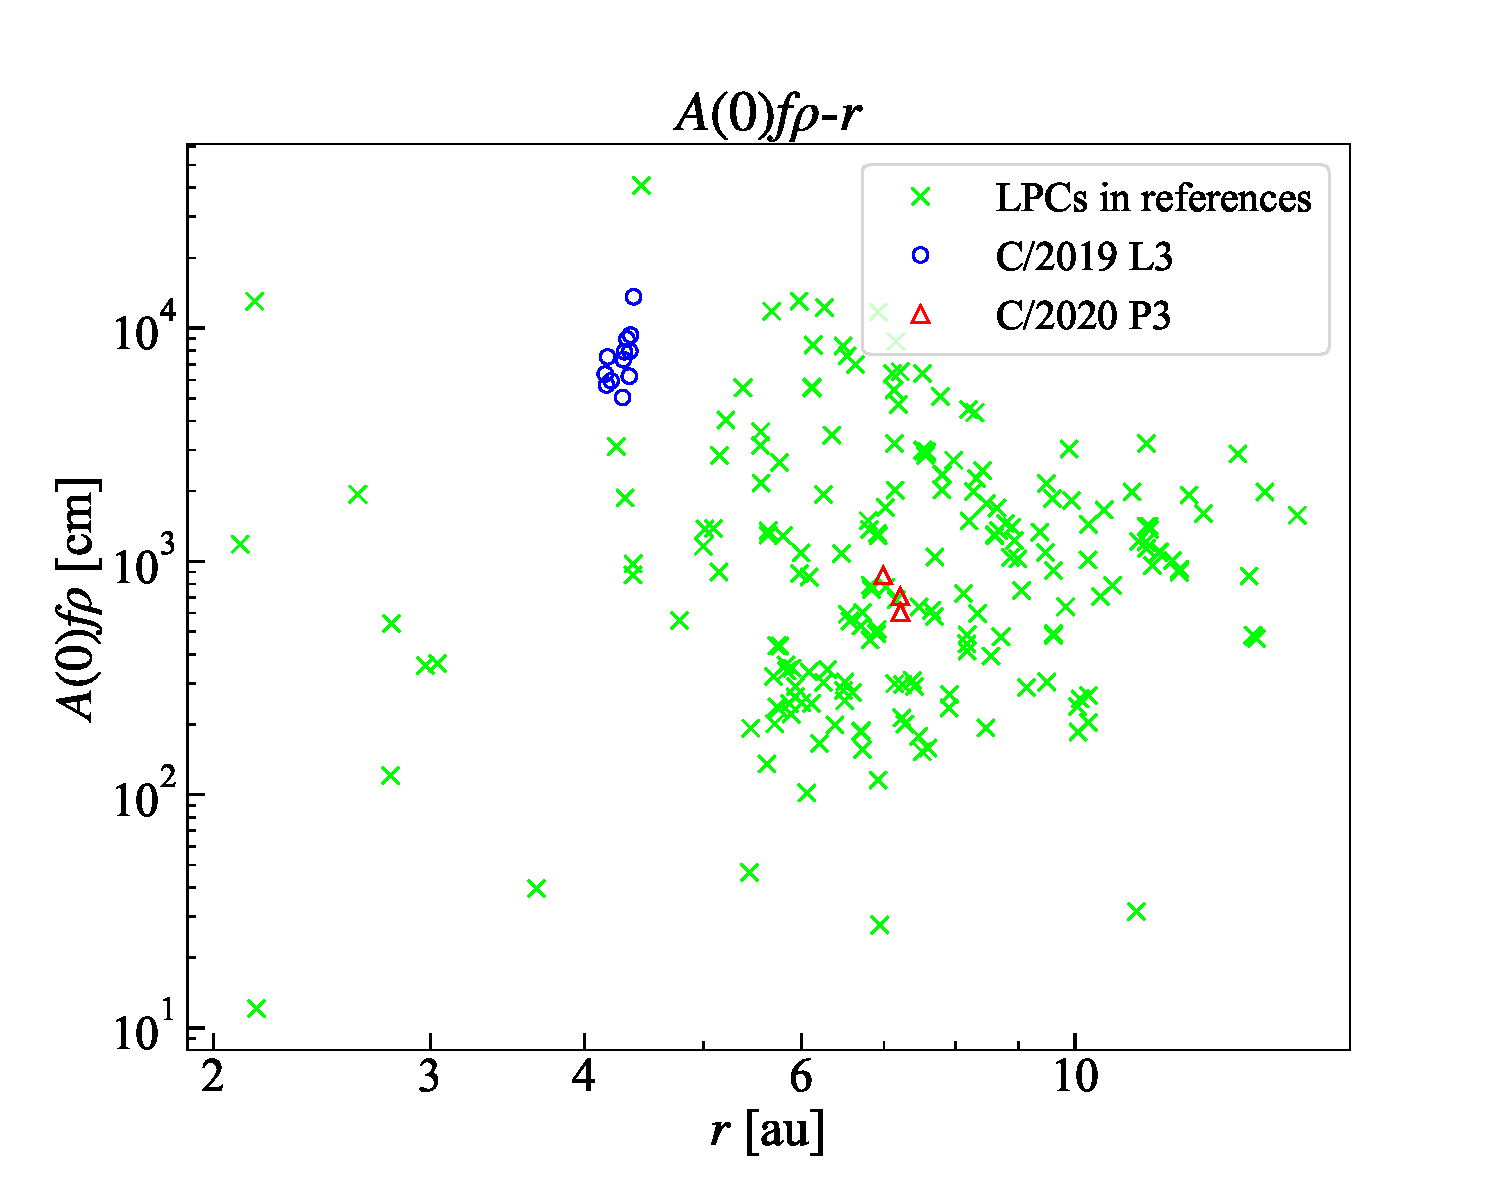
\includegraphics[width=\columnwidth]{a0frho-r.pdf}
    \caption{$A(0)f\rho$ values measured in this work compared with that of other LPCs in  literature by \citet{mazzotta_epifani_observational_2014}, \citet{garcia_photometry_2021}, \citet{garcia_observational_2020}, \citet{rousselot_monitoring_2014}, \citet{meech_activity_2009}, \citet{sarneczky_activity_2016}, \citet{solontoi_ensemble_2012}, and \citet{szabo_spectrophotometry_2002}. All data have been adjusted to phase angle \ang{0}. }\label{fig:afrho-ref}
\end{figure}

\begin{figure}
    \centering
    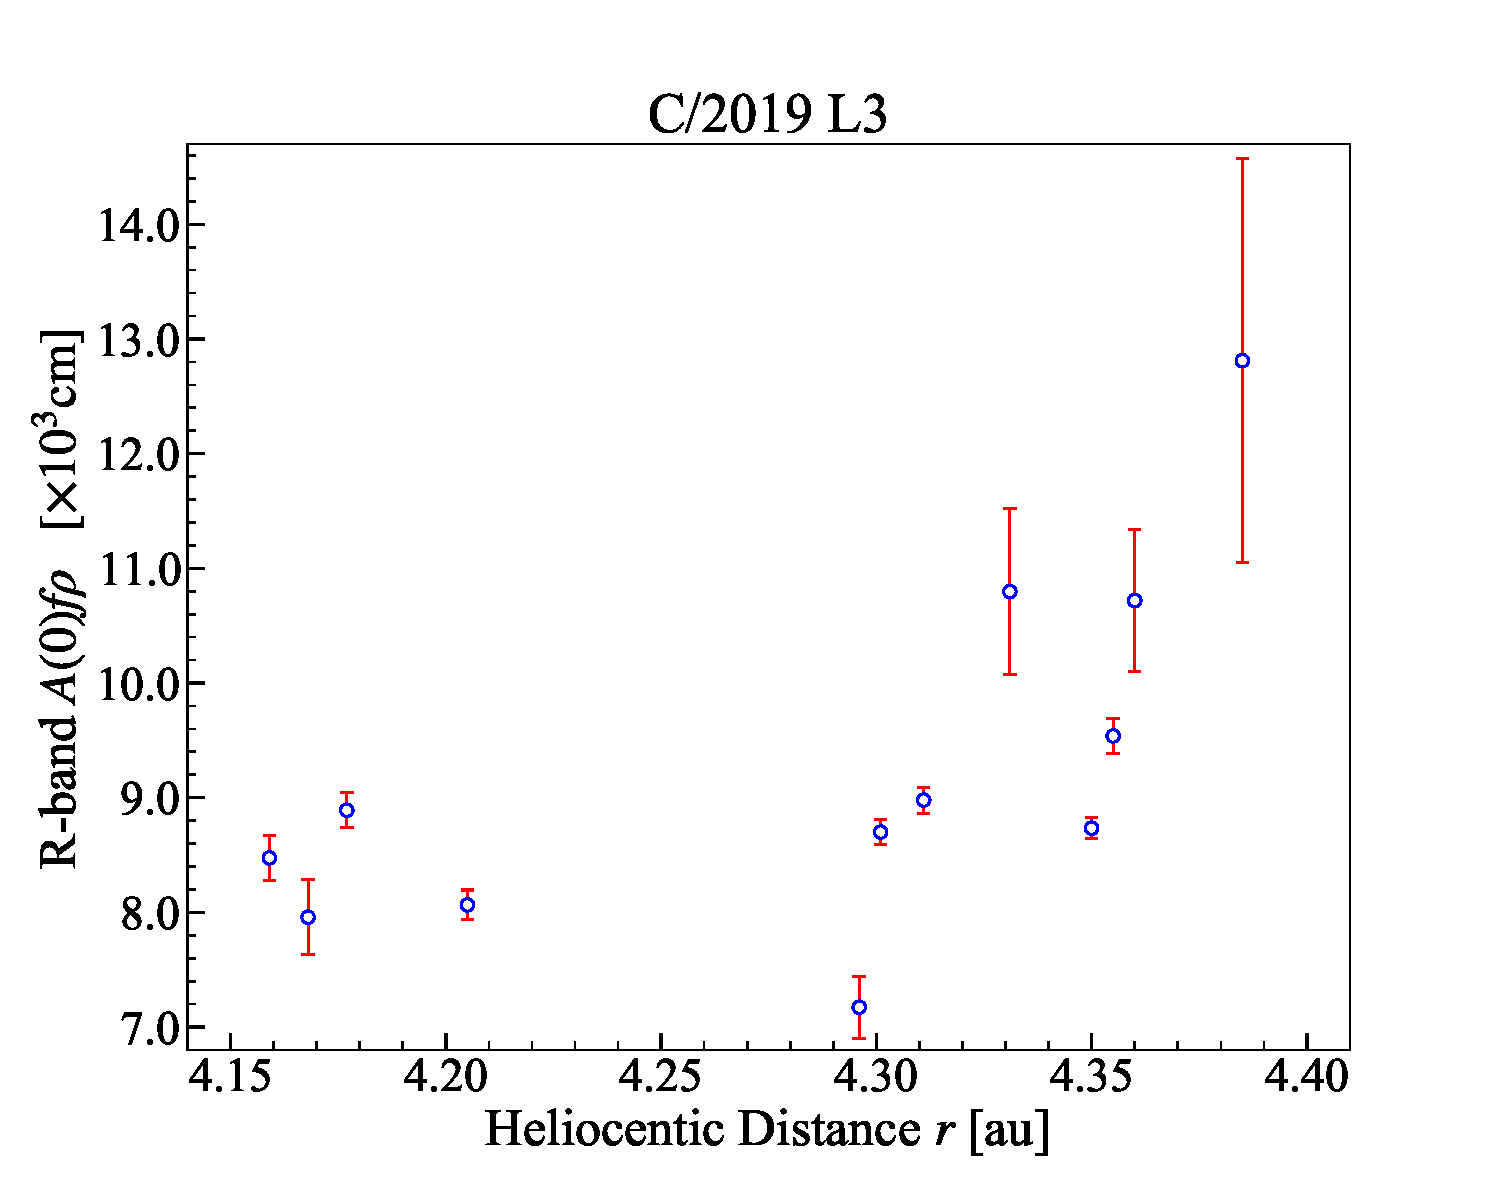
\includegraphics[width=\columnwidth]{a0frho-r-C2019L3-new.pdf}
    \caption{R-band $A(0)f\rho$ values of C/2019 L3 (ATLAS) as a function of heliocentric distance. }\label{fig:a0frho-c2019}
\end{figure}

According to the study by \cite{ramirez_ubvric_2012}, the solar colors are as follows: 
${(\mathrm{B-V})}_{\odot} = \num{0.653 +- 0.005}$, 
${(\mathrm{V-R})}_{\odot} = \num{0.352 +- 0.007}$, and 
${(\mathrm{R-I})}_{\odot} = \num{0.350 +- 0.009}$. 
The average color indices of two Long-period comets and three dynamically new comets were calculated by \cite{meech_activity_2009} to be 
$\langle \mathrm{B-V} \rangle = \num{0.76 +- 0.01}$ and 
$\langle \mathrm{V-R} \rangle = \num{0.43 +- 0.01}$, 
with their heliocentric distances ranging from \qtyrange{5.8}{14.0}{\astronomicalunit}. 
\cite{solontoi_ensemble_2012} studied six Long-period comets within \qty{5}{\astronomicalunit} of the Sun and obtained the color indices of 
$\langle \mathrm{B-V} \rangle = \num{0.687 +- 0.005}$ and 
$\langle \mathrm{V-R} \rangle = \num{0.443 +- 0.003}$. 
\cite{jewittCOLORSYSTEMATICSCOMETS2015} investigated Long-period comets with large range of heliocentric distances (\qtyrange{1.875}{17.982}{\astronomicalunit}), and the color indices were found to be 
$\langle \mathrm{B-V} \rangle = \num{0.78 +- 0.02}$, 
$\langle \mathrm{V-R} \rangle = \num{0.47 +- 0.02}$, and 
$\langle \mathrm{R-I} \rangle = \num{0.42 +- 0.03}$. 

Fig.~\ref{fig:color-color} is the $\langle \mathrm{B-V} \rangle$ versus $\langle \mathrm{V-R} \rangle$ plot of C/2019 L3, C/2020 P3 and other LPCs. 
The color index of the Sun \citep{ramirez_ubvric_2012} is marked as a red circle with dot. 
As we can see, the $\langle \mathrm{B-V} \rangle$ colors of two comets are redder than the Sun, while the $\langle \mathrm{V-R} \rangle$ colors of them are bluer than the Sun. 
Compared with LPCs in other works, the $\langle \mathrm{B-V} \rangle$ color of C/2019 L3 is consistent with them, while the $\langle \mathrm{V-R} \rangle$ color of C/2019 L3 is significantly bluer than them. For C/2020 P3, the $\langle \mathrm{B-V} \rangle$ color is redder while the $\langle \mathrm{V-R} \rangle$ color is bluer. 
In general, the color indices of the two LPCs studied in this work differ from those of other LPCs. 

\begin{figure}
    \centering
    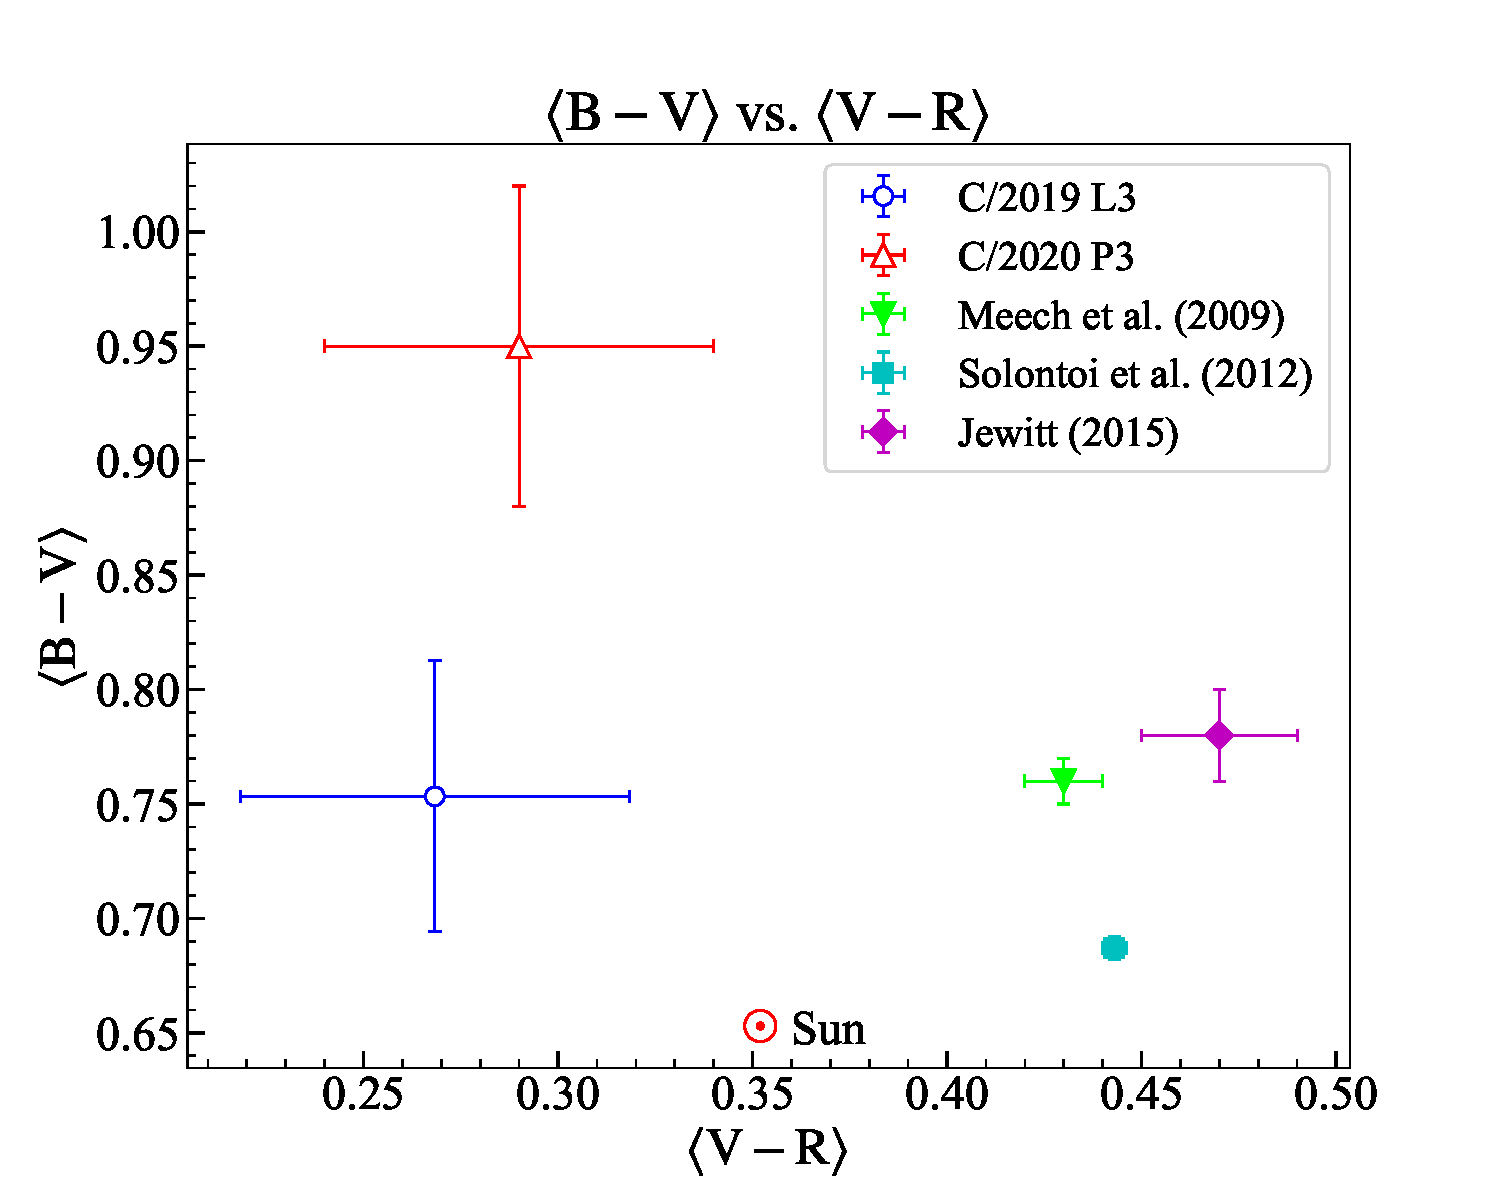
\includegraphics[width=\linewidth]{color-color.pdf}
    \caption{Color indices $\langle \mathrm{B-V} \rangle$ vs. $\langle \mathrm{V-R} \rangle$ plot of Long-period comets}.\label{fig:color-color}
\end{figure}

Cometary colors may vary with photometric aperture, and numerous studies have explored this dependence (e.g., \citealt{betzler_analysis_2017}; \citealt{kolokolova_color_2003}). In order to maximize the color differences with apertures, the $\mathrm{B-R}$ color is well-suited for analysis \citep{jewittCOLORSYSTEMATICSCOMETS2015}. For this purpose, the $\mathrm{B-R}$ color of the two comets is additionally measured with variable apertures, and some of the results are shown in Fig.~\ref{fig:color-aper}, where linear regression on the $\mathrm{B-R}$-aperture region is performed around \qty{40000}{\km}, and the slope of the fitting line (blue dashed line) is used to quantify the $\mathrm{B-R}$ color variation. The fitting errors are all omitted since they are negligible. Table~\ref{tab:color-variation} lists the $\mathrm{B-R}$ color variations in units of [\unit{mag/\qty{e4}{\km}}] for comets C/2019 L3 and C/2020 P3. For comet C/2019 L3, the $\mathrm{B-R}$ color variations are very small, with an average value of \qty{-8.93e-3}{mag/\qty{e4}{\km}}, and in most cases, its $\mathrm{B-R}$ color becomes bluer as the aperture size increases. For comet C/2020 P3, the $\mathrm{B-R}$ color observed on \DTMdate{2021-5-12}, displays a relatively larger variation with aperture size, with a fitting slope reaching \qty{0.38}{mag/\qty{e4}{\km}}. The shift towards a bluer coma color with increasing aperture size is attributed to variations in the size sorting of dust particles or changes in composition relative to cometocentric distance \citep{kolokolova_physical_2004}. Conversely, the sublimation of water ice can contribute to a redder coma color with larger apertures \citep{kolokolova_color_2003}. 


\begin{figure}
    \centering
    \subcaptionbox{\DTMdate{2021-4-4}}[.48\linewidth]{
        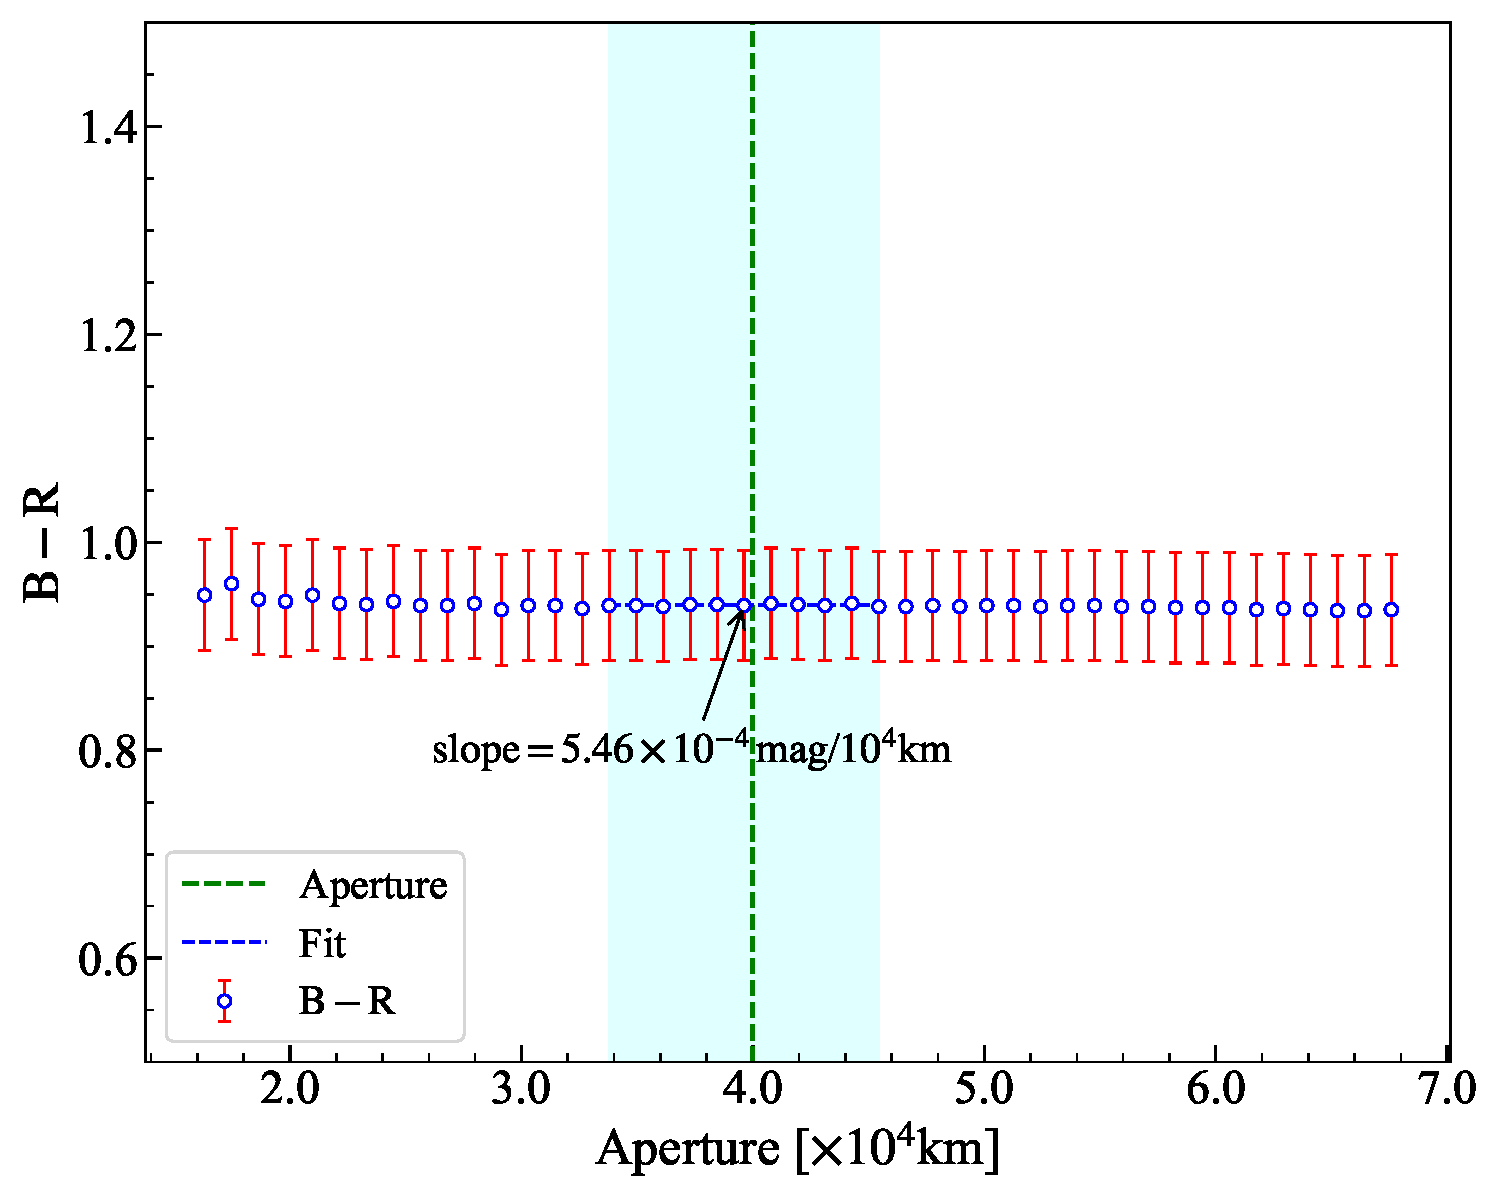
\includegraphics[width=\linewidth]{BminusR-rho-C2019L3-210404.pdf}
    }
    \subcaptionbox{\DTMdate{2021-4-8}}[.48\linewidth]{
        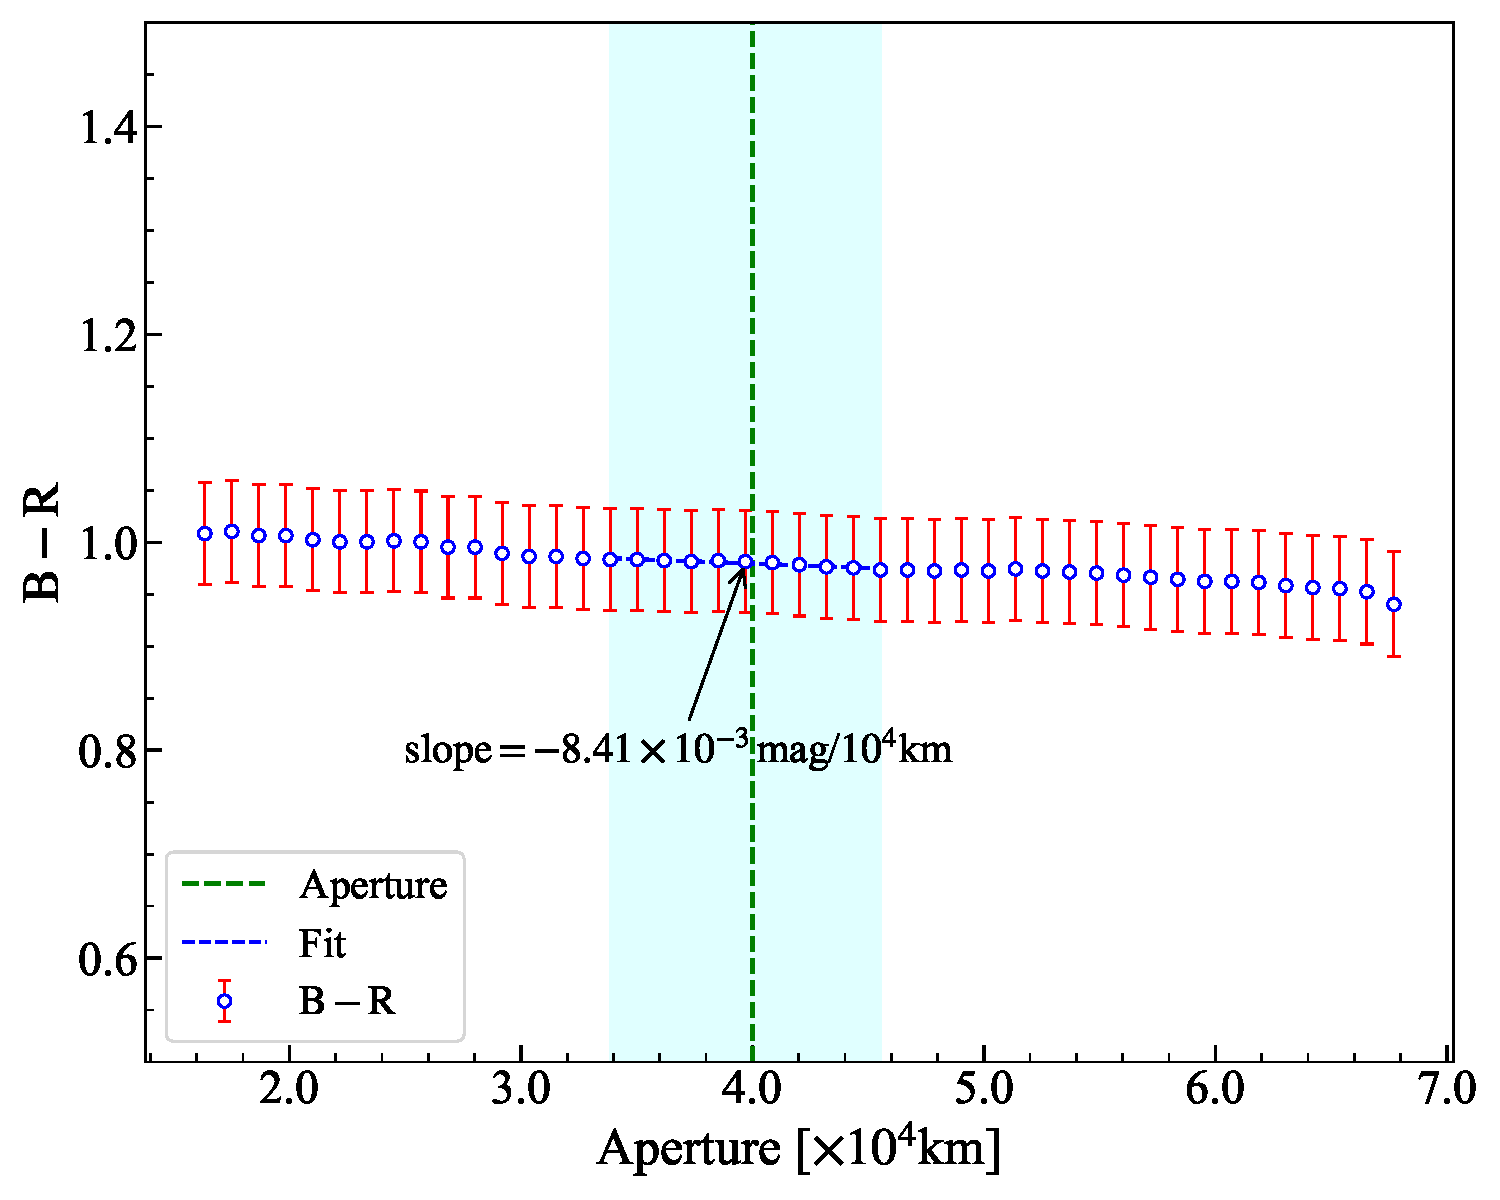
\includegraphics[width=\linewidth]{BminusR-rho-C2019L3-210408.pdf}
    }
    \subcaptionbox{\DTMdate{2021-4-12}}[.48\linewidth]{
        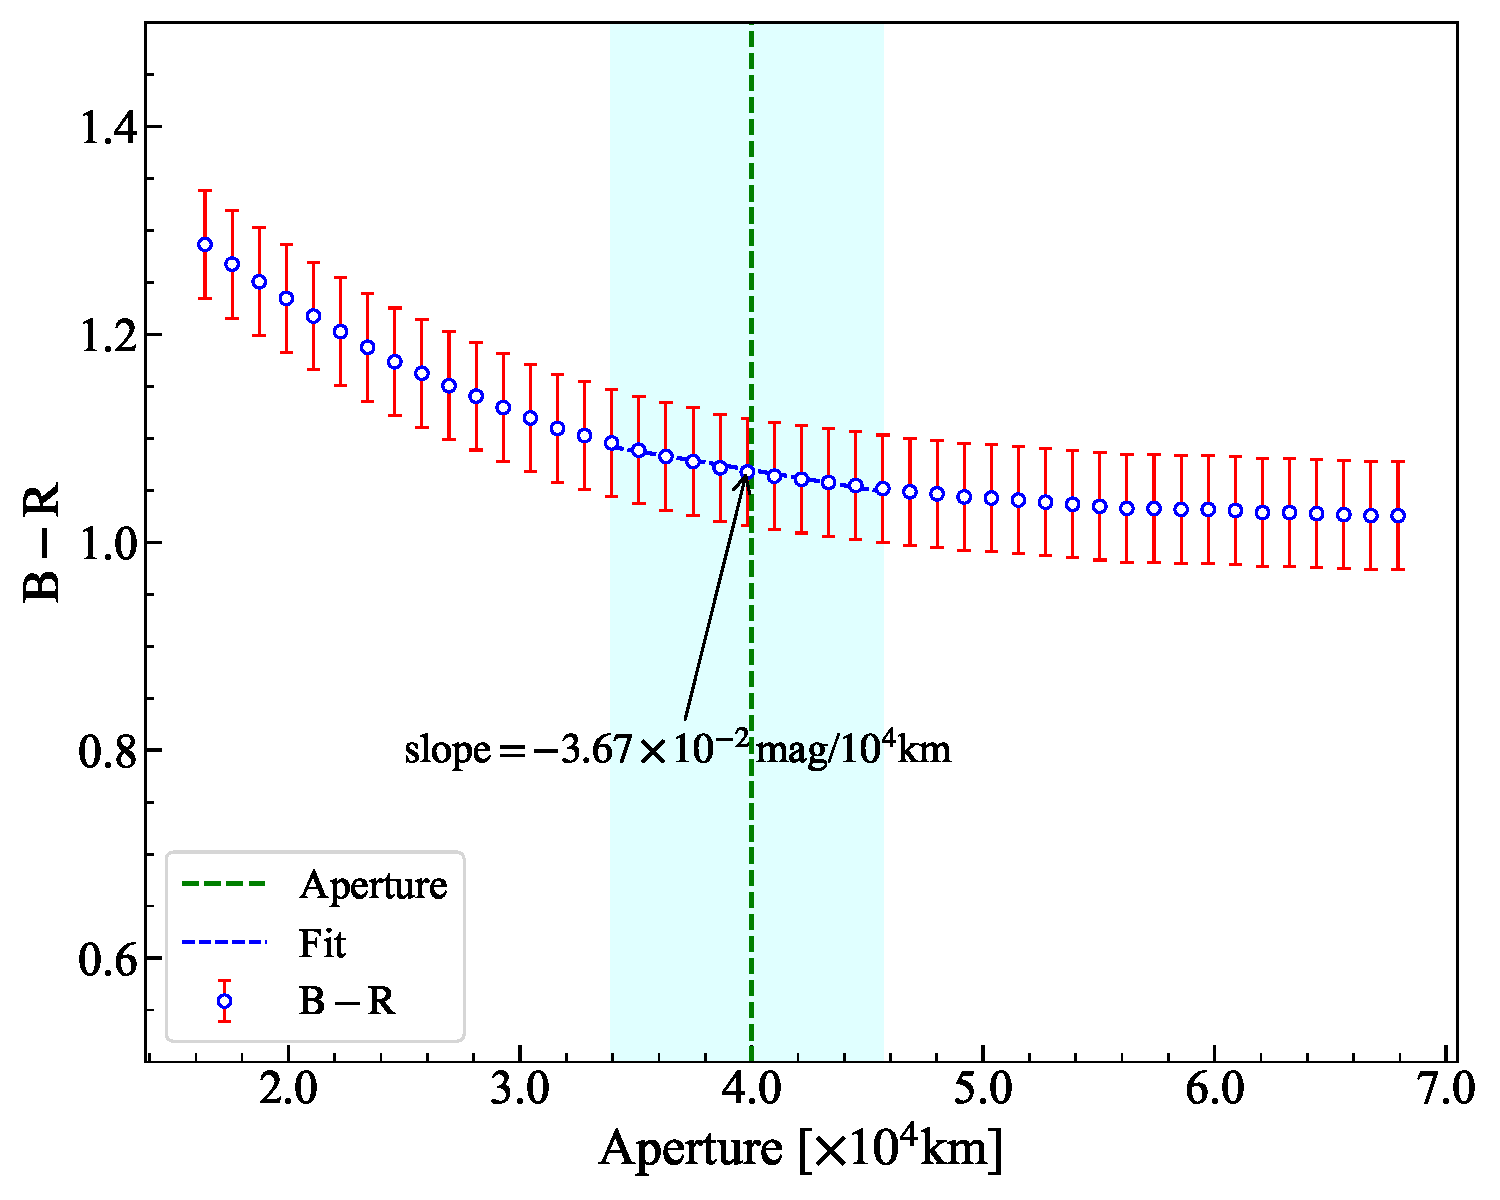
\includegraphics[width=\linewidth]{BminusR-rho-C2019L3-210412.pdf}
    }
    \subcaptionbox{\DTMdate{2021-5-14}}[.48\linewidth]{
        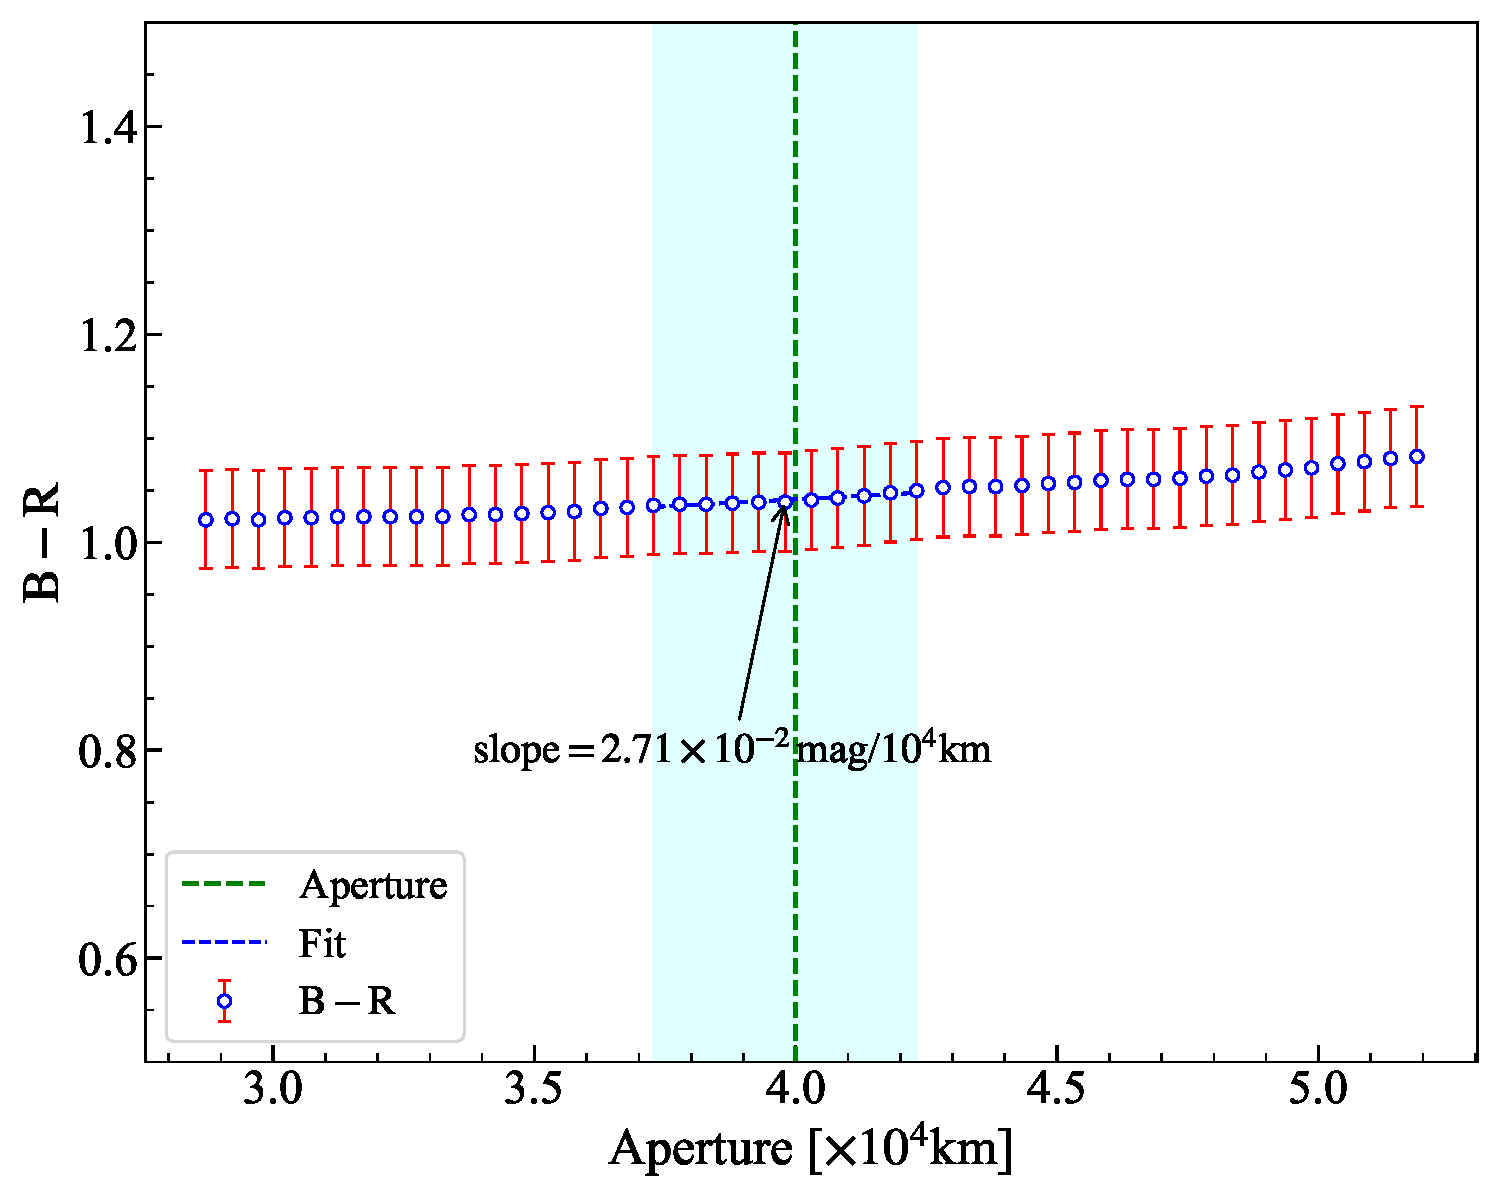
\includegraphics[width=\linewidth]{BminusR-rho-C2019L3-210514-095.pdf}
    }
    \caption{$\mathrm{B-V}$ color as a function of aperture for comet C/2019 L3. The green dashed line at {\qty{40000}{\km}} represents photometric aperture used in Section~\ref{sec:data-reduction}. Least squares fittig is performed on the cyan region around {\qty{40000}{\km}}, and the slope of fit is used to quantify color variation. }
    \label{fig:color-aper}
\end{figure}

\begin{table}
    \centering
    \caption{$\mathrm{B-R}$ color variations around photometric aperture for comets C/2019 L3 (ATLAS) and C/2020 P3 (ATLAS).}\label{tab:color-variation}
    \begin{threeparttable}
        \begin{tabular}{cc}
            \toprule
            Observation Time & $\mathrm{B-R}$ color variation [\unit{mag/\qty{e4}{\km}}] \\
            \midrule
            \multicolumn{2}{l}{\textbf{C/2019 L3 (ATLAS)}} \\
            2021-03-28.729 & \num{-3.87e-2} \\
            2021-04-02.739 & \num{-4.53e-3} \\
            2021-04-03.719 & \num{-5.62e-3} \\
            2021-04-04.691 & \num{5.46e-4} \\
            2021-04-08.691 & \num{-8.41e-3} \\
            2021-04-12.724 & \num{-3.67e-2} \\
            2021-04-14.702 & \num{-2.16e-2} \\
            2021-04-15.714 & \num{-2.56e-3} \\
            2021-05-04.736 & \num{4.50e-3} \\
            2021-05-10.735 & \num{-1.56e-2} \\
            2021-05-12.724 & \num{-5.49e-3} \\
            2021-05-14.721 & \num{2.71e-2} \\
            \multicolumn{2}{l}{\textbf{C/2020 P3 (ATLAS)}} \\
            2021-05-12.749 & \num{3.80e-1} \\
            \bottomrule
        \end{tabular}
    \end{threeparttable}
\end{table}

In summary, we present the observational results of comets C/2019 L3 and C/2020 P3. The conclusions are as follows: 
\begin{enumerate}
    \item The average gradient value of the surface brightness profile of comet C/2019 L3 is \num{-1.60}, suggesting a nonsteady coma. 
    \item The R-band $A(0)f\rho$ values of C/2019 L3 range from {\qty{5043 +- 244}{\cm}} to {\qty{13611 +- 1874}{\cm}}, and those of C/2020 P3 range from {\qty{606 +- 31}{\cm}} to {\qty{869 +- 20}{\cm}}. Compared to other works, the $A(0)f\rho$ of C/2019 L3 is relatively high at $\thicksim${\qty{4}{\astronomicalunit}}, while that of C/2020 P3 is moderate at $\thicksim${\qty{7}{\astronomicalunit}}. The R-band $A(0)f\rho$ values of C/2019 L3 tend to decrease first and then increase, so it is possible that comet C/2019 L3 experienced an outburst event in the past, and it was still active after this stage. 
    \item The colors of C/2019 L3 are  
        $\langle \mathrm{B-V} \rangle = \num{0.75 +- 0.06}$, 
        $\langle \mathrm{V-R} \rangle = \num{0.28 +- 0.05}$, and 
        $\langle \mathrm{R-I} \rangle = \num{0.21 +- 0.05}$,  
        while the colors of C/2020 P3 are 
        $\mathrm{B-V} = \num{1.04 +- 0.09}$, 
        $\langle \mathrm{V-R} \rangle = \num{0.26 +- 0.05}$, and 
        $\mathrm{R-I} = \num{0.76 +- 0.04}$. 
        The $\mathrm{B-V}$ colors of C/2019 L3 and C/2020 P3 are redder than the Sun, while the $\mathrm{V-R}$ and $\mathrm{R-I}$ colors of them are bluer than the Sun. Compared to other Long-period comets, both C/2019 L3 and C/2020 P3 exhibit distinct differences in their color indices. 
    \item For comet C/2019 L3, its color exhibits slight variation with photometric aperture. From the observation on \DTMdate{2021-5-12}, it can be observed that the color of comet C/2020 P3 becomes redder as the photometric aperture enlarges, which may be related to the sublimation of water ice. 
    \item The reddening of C/2019 L3 calculated from B-band $Af\rho$ and R-band $Af\rho$ exhibits variations during the observational runs, from {\qty{13.75 +- 1.07}{\percent/\kilo\angstrom}} to {\qty{-15.69 +- 0.37}{\percent/\kilo\angstrom}} with an average value of {\qty{0.94 +- 0.23}{\percent/\kilo\angstrom}}. This could be attributed to  variations in the composition of the coma. As for C/2020 P3, the reddening could only be calculated for the date of \DTMdate{2021-5-12}, yielding a value of {\qty{-6.65 +- 0.01}{\percent/\kilo\angstrom}}. 
\end{enumerate}
